% \begin{savequote}[75mm] 
% This is some random quote to start off the chapter.
% \qauthor{Firstname lastname} 
% \end{savequote}
\chapter{Dữ liệu}
\section{Giới thiệu bộ dữ liệu}

Bộ dữ liệu được sử dụng trong bài báo là dữ liệu về giá Bitcoin hàng ngày, thu thập từ ngày 31 tháng 3 năm 2015 đến ngày 1 tháng 4 năm 2022. Dữ liệu được tác giả lấy từ nhiều nguồn uy tín về đầu tư và tài chính như \textit{Yahoo Finance}, \textit{Coinmarketcap.com}, \textit{Investing.com}, \textit{Bitinfocharts.com}, và \textit{Coinmetrics.io}. 

Dữ liệu bao gồm tổng cộng 47 biến, được sử dụng để dự đoán giá Bitcoin trong tương lai. Các biến này được chia thành tám nhóm chính như sau:

\begin{itemize}
    \item \textbf{(a)} Các biến về giá Bitcoin
    \item \textbf{(b)} Đặc trưng kỹ thuật của Bitcoin
    \item \textbf{(c)} Các loại tiền mã hóa khác
    \item \textbf{(d)} Hàng hóa
    \item \textbf{(e)} Các chỉ số thị trường
    \item \textbf{(f)} Tỷ giá ngoại hối
    \item \textbf{(g)} Mức độ quan tâm của công chúng
    \item \textbf{(h)} Các biến giả cho các ngày trong tuần
\end{itemize}

Bảng \ref{tab:definition_variables} dưới đây giải thích ý nghĩa từng biến trong bộ dữ liệu. Biến mục tiêu của bộ dữ liệu là giá đóng cửa hàng ngày của Bitcoin, được biểu diễn bằng biến \textbf{BTC\_Close} và tính bằng USD.

\begin{table}[h]
    \centering
    \resizebox{\textwidth}{!}{
    \begin{tabular}{|l|l|}
        \hline
        \textbf{Biến} & \textbf{Mô tả} \\ \hline
        \multicolumn{2}{|c|}{\textbf{(a) Bitcoin}} \\ \hline
        BTC\_Open & Giá mở cửa của Bitcoin \\ \hline
        BTC\_Close & Giá đóng cửa của Bitcoin \\ \hline
        BTC\_High & Giá cao nhất trong ngày của Bitcoin \\ \hline
        BTC\_Low & Giá thấp nhất trong ngày của Bitcoin \\ \hline
        BTC\_Volume & Khối lượng giao dịch Bitcoin \\ \hline
        \multicolumn{2}{|c|}{\textbf{(b) Đặc trưng kỹ thuật của Bitcoin}} \\ \hline
        Active addr cnt & Số lượng địa chỉ hoạt động \\ \hline
        Xfer cnt & Số lượng chuyển giao \\ \hline
        Mean Tx size & Kích thước trung bình của giao dịch \\ \hline
        Total fees (USD) & Tổng phí giao dịch (USD) \\ \hline
        Mean hash rate & Tốc độ băm trung bình \\ \hline
        Difficulty & Độ khó khai thác \\ \hline
        Mean block size (bytes) & Kích thước khối trung bình (bytes) \\ \hline
        Sum block weight & Tổng trọng lượng khối \\ \hline
        \multicolumn{2}{|c|}{\textbf{(c) Các loại tiền mã hóa khác}} \\ \hline
        LTC & Giá Litecoin (USD) \\ \hline
        XRP & Giá Ripple (USD) \\ \hline
        DASH & Giá Dash (USD) \\ \hline
        DOGE & Giá Dogecoin (USD) \\ \hline
        ETH & Giá Ethereum (USD) \\ \hline
        \multicolumn{2}{|c|}{\textbf{(d) Hàng hóa}} \\ \hline
        Gold & Giá vàng (USD/ounce) \\ \hline
        Silver & Giá bạc (USD/ounce) \\ \hline
        Copper & Giá đồng (USD/ounce) \\ \hline
        \multicolumn{2}{|c|}{\textbf{(e) Chỉ số thị trường}} \\ \hline
        S\&P500 & Chỉ số Standard and Poor's 500 \\ \hline
        DJI & Chỉ số Dow Jones Industrial Average \\ \hline
        CBOE & Chicago Board Options Exchange \\ \hline
        NASDAQ & National Association of Securities Dealers Automated Quotations \\ \hline
        JP225 & Nikkei 225 \\ \hline
        CSI300 & Chỉ số chứng khoán Trung Quốc CSI 300 \\ \hline
        \multicolumn{2}{|c|}{\textbf{(f) Tỷ giá ngoại hối}} \\ \hline
        DXY & Chỉ số Đô la Mỹ \\ \hline
        EUR & Tỷ giá Euro/USD \\ \hline
        GBP & Tỷ giá Bảng Anh/USD \\ \hline
        JPY & Tỷ giá Yên Nhật/USD \\ \hline
        CAD & Tỷ giá Đô la Canada/USD \\ \hline
        AUD & Tỷ giá Đô la Úc/USD \\ \hline
        SGD & Tỷ giá Đô la Singapore/USD \\ \hline
        CNY & Tỷ giá Nhân dân tệ/USD \\ \hline
        RUB & Tỷ giá Rúp Nga/USD \\ \hline
        \multicolumn{2}{|c|}{\textbf{(g) Mức độ quan tâm của công chúng}} \\ \hline
        Google & Xu hướng tìm kiếm trên Google \\ \hline
        Tweets & Số lượng tweet hàng ngày \\ \hline
        \multicolumn{2}{|c|}{\textbf{(h) Tuần}} \\ \hline
        Monday--Sunday & Biến giả cho các ngày trong tuần \\ \hline
    \end{tabular}}
    \caption{Ý nghĩa các biến}
    \label{tab:definition_variables}
\end{table}

\clearpage

\section{Khám phá dữ liệu - EDA}

Bảng \ref{tab:explanatory_variables} trình bày các đặc điểm thống kê của từng biến được sử dụng để dự đoán giá Bitcoin trong bài toán. 

\begin{table}[h]
    \centering
    \resizebox{\textwidth}{!}{
    \begin{tabular}{|l|r|r|r|r|}
        \hline
        \textbf{Biến} & \textbf{Số lượng} & \textbf{Giá trị trung bình} & \textbf{Độ lệch chuẩn} & \textbf{Giá trị nhỏ nhất / lớn nhất} \\ \hline
        BTC\_Open & 2559 & 12,628.14 & 16,689.78 & 210.07 / 67,549.73 \\ \hline
        BTC\_High & 2559 & 12,965.49 & 17,133.74 & 223.83 / 68,789.63 \\ \hline
        BTC\_Low & 2559 & 12,259.05 & 16,184.48 & 199.57 / 66,382.06 \\ \hline
        BTC\_Close & 2559 & 12,644.27 & 16,697.06 & 210.49 / 67,566.83 \\ \hline
        BTC\_Volume & 2559 & $1.6 \times 10^{10}$ & $2.02 \times 10^{10}$ & 10,600,903 / $5.4 \times 10^{11}$ \\ \hline
        Active addr cnt & 2559 & 715,123 & 235,979.6 & 226,902 / 1,264,064 \\ \hline
        Xfer cnt & 2559 & 646,493.3 & 183,825.9 & 234,806 / 2,041,653 \\ \hline
        Mean Tx size (native units) & 2559 & 2.092273 & 3.50753 & 0.307039 / 126.7199 \\ \hline
        Total fees (USD) & 2559 & 936,734.4 & 1,971,955 & 2850.355 / 21,297,763 \\ \hline
        Mean hash rate & 2559 & 60,571.48 & 61,650.19 & 271,738.1 / $2.48 \times 10^5$ \\ \hline
        Difficulty & 2559 & $8.37 \times 10^{12}$ & $8.5 \times 10^{12}$ & $4.67 \times 10^{11}$ / $2.86 \times 10^{13}$ \\ \hline
        Mean block size (in bytes) & 2559 & 986,516.8 & 285,461.9 & 292,293.9 / 1,238,861 \\ \hline
        Sum block weight & 2559 & $4.82 \times 10^8$ & $1.05 \times 10^8$ & $1.91 \times 10^5$ / $7.58 \times 10^8$ \\ \hline
        LTC & 2559 & 71.87075 & 70.81633 & 1.32117 / 386.4508 \\ \hline
        XRP & 2559 & 0.354487 & 0.38141 & 0.00356 / 2.78 \\ \hline
        DASH & 2559 & 142.1313 & 182.4392 & 2.06 / 1550.85 \\ \hline
        DOGE & 2559 & 0.035873 & 0.087754 & $8.73 \times 10^{-5}$ / 0.6848 \\ \hline
        ETH & 2430 & 708.8693 & 1107.578 & 0.4348 / 4812.09 \\ \hline
        Gold & 1854 & 1489.887 & 245.8335 & 1070.8 / 2117.1 \\ \hline
        Silver & 2182 & 19.18016 & 3.757016 & 11.978 / 30.135 \\ \hline
        Copper & 1811 & 3.00615 & 0.697527 & 1.994 / 4.9375 \\ \hline
        Oil & 1848 & 54.88971 & 14.53394 & -37.63 / 123.7 \\ \hline
        Treasury yield 10 years & 1763 & 1.950953 & 0.657184 & 0.499 / 3.2434 \\ \hline
        S\&P500 & 1766 & 2907.096 & 779.8341 & 1829.08 / 4796.56 \\ \hline
        DJI & 1766 & 24,828.27 & 5703.945 & 15,660.18 / 36,799.65 \\ \hline
        CBOE & 1765 & 94.984 & 21.60072 & 55.5 / 137.16 \\ \hline
        NASDAQ & 1765 & 8336.731 & 3308.791 & 4266.84 / 16,057.44 \\ \hline
        JP225 & 1740 & 21,972.35 & 3738.272 & 14,952.02 / 30,670.1 \\ \hline
        CSI300 & 1708 & 392.53 & 668.6175 & 2853.76 / 5807.72 \\ \hline
        DXY & 1764 & 95.63923 & 2.961022 & 88.59 / 103.29 \\ \hline
        EUR & 1826 & 1.343444 & 0.081068 & 1.114939 / 1.558512 \\ \hline
        GBP & 1826 & 0.747114 & 0.046768 & 0.62952 / 0.86999 \\ \hline
        JPY & 1826 & 111.051 & 5.136474 & 99.906 / 125.629 \\ \hline
        CAD & 1826 & 1.303631 & 0.04442 & 1.1954 / 1.4578 \\ \hline
        AUD & 1826 & 1.367315 & 0.07251 & 1.232 / 1.741281 \\ \hline
        SGD & 1826 & 1.362716 & 0.029435 & 1.30659 / 1.4563 \\ \hline
        CNY & 1826 & 0.733239 & 0.037271 & 0.57429 / 0.811688 \\ \hline
        RUB & 1826 & 66.58596 & 8.73112 & 47.196 / 138.9651 \\ \hline
        Tweets & 2559 & 50,500.83 & 43,438.57 & 13,294 / 363,425 \\ \hline
        Google & 2559 & 495.8206 & 519.2102 & 64 / 6064.5 \\ \hline
    \end{tabular}}
    \caption{Đặc điểm thống kê của các biến}
    \label{tab:explanatory_variables}
\end{table}

\clearpage

Đáng chú ý, các biến liên quan đến thị trường tiền mã hóa, bao gồm năm biến về giá Bitcoin, năm biến dành cho các loại tiền mã hóa khác như LTC, XRP, DASH, DOGE, ETH và cả khối lượng tìm kiếm trên Google về Bitcoin, đều có độ lệch chuẩn rất cao. Điều này cho thấy sự dao động lớn trong các dữ liệu thu thập được, đặc biệt là trong thị trường tiền mã hóa. Điểm đáng lưu ý là tỷ lệ giữa độ lệch chuẩn và giá trị trung bình (hệ số biến thiên - coefficient of variation) của các biến này, ngoại trừ LTC với tỷ lệ 0.99, đều vượt quá 1. Điều này chứng tỏ rằng thị trường tiền mã hóa từ năm 2015 đến nay đã trải qua những biến động mạnh mẽ và không ngừng, với mức độ dao động lớn hơn nhiều so với các thị trường tài chính truyền thống.

Sự chênh lệch lớn trong tỷ lệ này so với các biến thuộc thị trường truyền thống (với tỷ lệ không vượt quá 0.4) càng làm nổi bật tính bất ổn của thị trường tiền mã hóa. Trong khi đó, các biến của thị trường truyền thống, bao gồm chỉ số chứng khoán (như S\&P 500, Dow Jones Industrial Average), hàng hóa (như vàng, bạc, dầu), và tỷ giá ngoại hối (như EUR/USD, JPY/USD), cho thấy mức độ biến động thấp hơn đáng kể, phản ánh tính ổn định hơn của các thị trường này.

Điều này không chỉ khẳng định rằng thị trường tiền mã hóa mang tính rủi ro cao hơn, mà còn phản ánh một đặc điểm cơ bản của nó: khả năng phản ứng mạnh mẽ với các tin tức và sự kiện toàn cầu, tâm lý nhà đầu tư, và xu hướng thị trường chung. Mức độ biến động cao của thị trường tiền mã hóa có thể được giải thích một phần bởi tính mới mẻ, chưa được kiểm soát hoàn toàn, và sự phụ thuộc lớn vào nhu cầu thị trường tức thời, so với các thị trường truyền thống đã có lịch sử lâu đời và có các cơ chế ổn định hơn.

Sự khác biệt giữa các biến giải thích của thị trường tiền mã hóa và thị trường truyền thống có thể được thấy rõ ràng thông qua tỷ lệ giữa giá trị nhỏ nhất và lớn nhất. Trong các biến của thị trường truyền thống, ngoại trừ đồng rúp Nga có tỷ lệ lớn nhất/nhỏ nhất là 194 lần, các tỷ lệ này không vượt quá 7, thậm chí khi tính đến cú sốc giá dầu thô vào ngày 20 tháng 4 năm 2020, khi giá dầu rơi xuống mức âm kỷ lục là -37,63 USD. Ngược lại, trong thị trường tiền mã hóa, tỷ lệ giữa giá trị lớn nhất và nhỏ nhất lại cực kỳ cao, đều vượt ngưỡng 300. Đặc biệt, Ethereum (ETH) có tỷ lệ lớn nhất/nhỏ nhất lên tới 11,067 lần, điều này cho thấy sự biến động vô cùng mạnh mẽ của đồng tiền này. Không chỉ Bitcoin, mà cả đồng rúp Nga cũng cho thấy mức độ biến động cao trong các thị trường này, mặc dù lý do biến động ở mỗi loại tài sản có thể khác nhau.

\newpage

\begin{figure}[h]
    \centering
    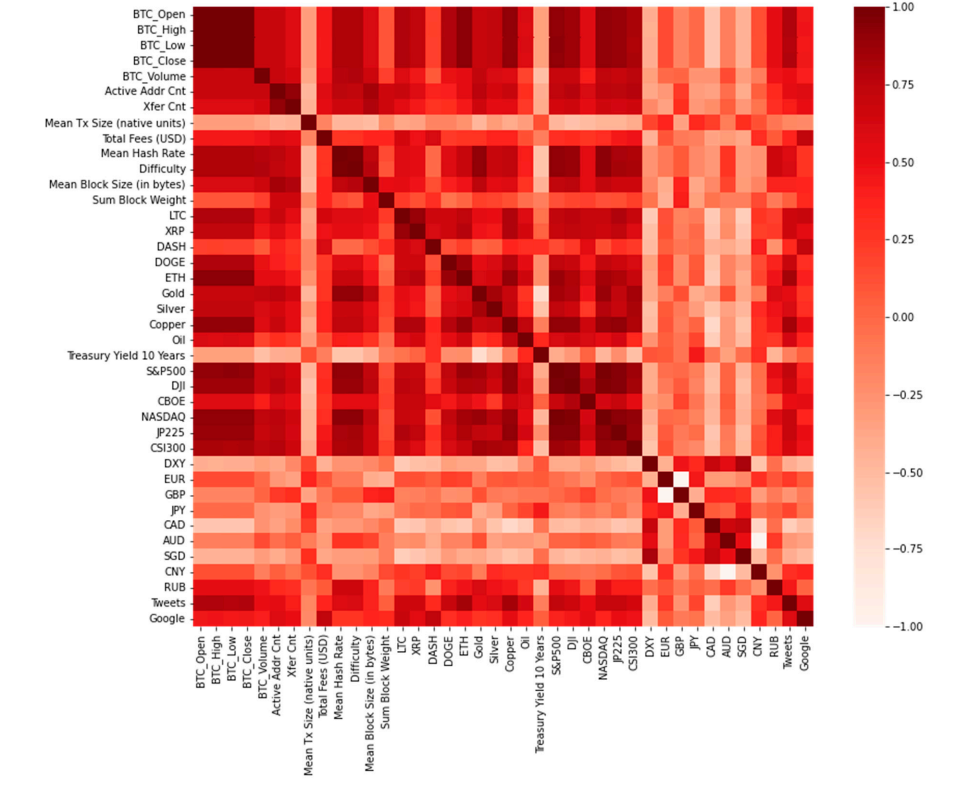
\includegraphics[width=\textwidth]{images/heatmap.png}
    \caption{Bản đồ nhiệt về mối tương quan giữa các biến}
    \label{fig:corr}
\end{figure}


Bản đồ nhiệt về mối tương quan (Hình \ref{fig:corr}) cho thấy Bitcoin có mối tương quan dương với nhiều loại tài sản khác, bao gồm các loại tiền mã hóa khác, giá hàng hóa, và các chỉ số thị trường chứng khoán. Điều này cho thấy rằng khi các thị trường này tăng trưởng, giá Bitcoin cũng có xu hướng tăng theo. Tuy nhiên, một điểm ngoại lệ quan trọng là mối tương quan nghịch giữa giá Bitcoin và lợi suất trái phiếu kho bạc Mỹ kỳ hạn 10 năm trong danh mục hàng hóa. Khi lợi suất trái phiếu tăng, giá Bitcoin có xu hướng giảm, điều này phản ánh dòng chảy vốn quay trở lại các tài sản an toàn hơn khi nền kinh tế có dấu hiệu cải thiện. Ngoài ra, mối tương quan âm giữa giá Bitcoin và tỷ giá hối đoái, đặc biệt là khi đồng USD mạnh lên, cũng là một xu hướng hợp lý, do giá trị của Bitcoin giảm khi đồng đô la trở nên hấp dẫn hơn. Điều đáng chú ý là tỷ giá đồng rúp Nga lại có mối tương quan dương cao với giá Bitcoin, có thể phản ánh tình trạng bất ổn kinh tế ở Nga dẫn đến việc dòng vốn dịch chuyển vào Bitcoin như một tài sản trú ẩn.

Một phát hiện thú vị khác là sự biến động của Bitcoin theo các ngày trong tuần. Biến động cực mạnh thường diễn ra vào thứ Tư, với phương sai lợi nhuận lớn nhất và những biến động hàng ngày lớn nhất, cả về tăng và giảm, đều xuất hiện vào ngày này. Ngược lại, vào cuối tuần, phương sai lợi nhuận giảm xuống và mức độ ổn định cao hơn so với các ngày trong tuần. Lợi nhuận trung bình hàng ngày của Bitcoin là 0,28\%, với biên độ tin cậy 95\% nằm trong khoảng [0,13\%, 0,43\%]. Đáng chú ý, lợi nhuận trung bình vào thứ Hai là cao nhất, trong khi vào Chủ Nhật là thấp nhất, cho thấy một xu hướng tăng giá mạnh vào đầu tuần. Xác suất tăng giá hàng ngày của Bitcoin là 54,57\%, với thứ Bảy và thứ Sáu là hai ngày có xác suất tăng cao nhất. Điều này cho thấy thị trường có những chu kỳ nhất định, có thể là do yếu tố giao dịch hoặc tác động từ các tin tức thị trường.

\begin{figure}[h]
    \centering
    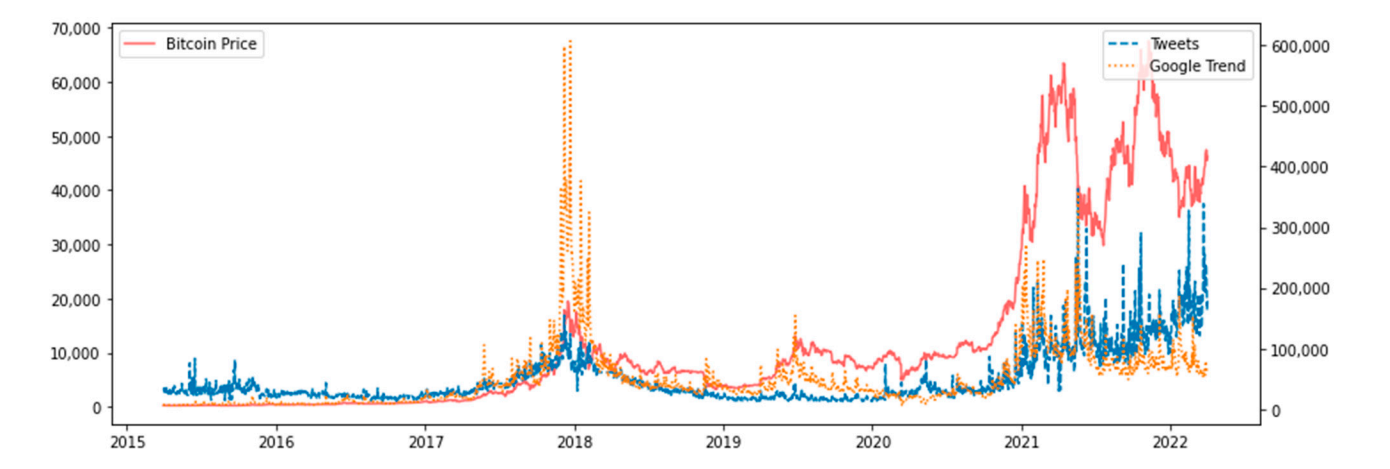
\includegraphics[width=\textwidth]{images/google_tweets_comparison.png}
    \caption{So sánh mức độ quan tâm của công chúng qua Google Trends và số lượng tweet hàng ngày với giá Bitcoin}
    \label{fig:interest_public}
\end{figure}

Liên quan đến mức độ quan tâm của công chúng, hai biến số quan trọng là xu hướng tìm kiếm trên Google và số lượng tweet hàng ngày (Hình \ref{fig:interest_public}) cũng có liên hệ chặt chẽ với biến động giá Bitcoin. Hai xu hướng chính có thể được rút ra: đầu tiên, đỉnh cao của Google Trends và số lượng tweet trùng khớp với những thời điểm Bitcoin đạt mức giá cao kỷ lục. Thứ hai, đỉnh cao nhất của Google Trends diễn ra vào cuối năm 2017, thời điểm Bitcoin đạt mốc giá quan trọng. Dù giá Bitcoin đã vượt ngưỡng 60.000 USD vào năm 2021, mức độ tìm kiếm trên Google vẫn không đạt đến đỉnh cao như năm 2017, cho thấy sự thay đổi trong mức độ quan tâm của công chúng đối với Bitcoin theo thời gian. Điều này có thể phản ánh sự bão hòa của thị trường tiền mã hóa hoặc sự thay đổi trong nhận thức của công chúng về Bitcoin.

